%% This is file `elsarticle-template-1-num.tex',
%%
%% Copyright 2009 Elsevier Ltd
%%
%% This file is part of the 'Elsarticle Bundle'.
%% ---------------------------------------------
%%
%% It may be distributed under the conditions of the LaTeX Project Public
%% License, either version 1.2 of this license or (at your option) any
%% later version.  The latest version of this license is in
%%    http://www.latex-project.org/lppl.txt
%% and version 1.2 or later is part of all distributions of LaTeX
%% version 1999/12/01 or later.
%%
%% The list of all files belonging to the 'Elsarticle Bundle' is
%% given in the file `manifest.txt'.
%%
%% Template article for Elsevier's document class `elsarticle'
%% with numbered style bibliographic references
%%
%% $Id: elsarticle-template-1-num.tex 149 2009-10-08 05:01:15Z rishi $
%% $URL: http://lenova.river-valley.com/svn/elsbst/trunk/elsarticle-template-1-num.tex $
%%
\documentclass[preprint,12pt]{elsarticle}

%% Use the option review to obtain double line spacing
%% \documentclass[preprint,review,12pt]{elsarticle}

%% Use the options 1p,twocolumn; 3p; 3p,twocolumn; 5p; or 5p,twocolumn
%% for a journal layout:
%% \documentclass[final,1p,times]{elsarticle}
%% \documentclass[final,1p,times,twocolumn]{elsarticle}
%% \documentclass[final,3p,times]{elsarticle}
%% \documentclass[final,3p,times,twocolumn]{elsarticle}
%% \documentclass[final,5p,times]{elsarticle}
%% \documentclass[final,5p,times,twocolumn]{elsarticle}

%% if you use PostScript figures in your article
%% use the graphics package for simple commands
%% \usepackage{graphics}
%% or use the graphicx package for more complicated commands
%% \usepackage{graphicx}
%% or use the epsfig package if you prefer to use the old commands
%% \usepackage{epsfig}

%% The amssymb package provides various useful mathematical symbols
\usepackage{amssymb}
%% The amsthm package provides extended theorem environments
%% \usepackage{amsthm}

%% The lineno packages adds line numbers. Start line numbering with
%% \begin{linenumbers}, end it with \end{linenumbers}. Or switch it on
%% for the whole article with \linenumbers after \end{frontmatter}.
%% \usepackage{lineno}

%% natbib.sty is loaded by default. However, natbib options can be
%% provided with \biboptions{...} command. Following options are
%% valid:

%%   round  -  round parentheses are used (default)
%%   square -  square brackets are used   [option]
%%   curly  -  curly braces are used      {option}
%%   angle  -  angle brackets are used    <option>
%%   semicolon  -  multiple citations separated by semi-colon
%%   colon  - same as semicolon, an earlier confusion
%%   comma  -  separated by comma
%%   numbers-  selects numerical citations
%%   super  -  numerical citations as superscripts
%%   sort   -  sorts multiple citations according to order in ref. list
%%   sort&compress   -  like sort, but also compresses numerical citations
%%   compress - compresses without sorting
%%
%% \biboptions{comma,round}

% \biboptions{}


\journal{Science of Computer Programming}

\usepackage{hyperref}
\usepackage{color}

\newcommand{\definition}[1]{ 
\begin{quote} \item {\em #1} \end{quote}}
\newcommand {\chaptersummary}[1] { \vspace{3cm} \hrule \vspace{0.5cm} {\em #1 } \vspace{0.5cm} \hrule \vspace{0.5cm} \newpage}
\newcommand{\challenge}[1]{\paragraph {\bf \em [Challenge]} {\em #1}} 



\newcommand{\chapquote}[1]{\em #1} 


\newcommand{\quest}[1]{{\em ({\bf Mircea:} #1)}}
\newcommand{\mir}[1]{{\em ({\bf Mircea:} #1)}}
\newcommand{\mircea}[1]{{\em ({\bf Mircea:} #1)}}
\newcommand{\Mircea}[1]{{\em ({\bf Mircea:} #1)}}

\newcommand{\pg}[2]{#1 #2}
%\newcommand{\pg}[2]{\paragraph {#1} {\small #2}}
\newcommand{\mic}[1]{{\small #1}}

\definecolor{lg}{rgb}{0.9,0.9,0.9}
\definecolor{darkblue}{rgb}{0.0,0.0,0.5}


\newcommand{\cbar}{\vspace {1cm} \hrule }

\newcommand{\concls}[1]{\titlebox{Facts and Limitations}{#1}}

\newcommand{\titlebox}[2]{
\vspace{1cm}
\hrule
\vspace{0.25cm}
{\bf #1: }
\vspace{0.25cm}
\hrule
#2
\vspace{0.5cm}
}


% Utils

\newcommand{\dpdef}[1]{\paragraph{Definition.} {\em #1}}
\newcommand{\dpdisc}[1]{\paragraph {Discussion.} #1}
\newcommand{\dpr}[1]{\paragraph {Rationale.} #1}
\newcommand{\dpcat}[1]{\paragraph {Category:} #1}
\newcommand{\dpcatage}{\dpcat{Age-related}}
\newcommand{\dpcatdyn}{\dpcat{Dynamics-related}}
\newcommand{\dpexample}[1]{\paragraph {Example.} #1}
\newcommand{\dpp}[1]{\newpage\subsection{#1}}


\newcommand{\pidea}[1]{#1.}
\newcommand{\pideap}[1]{#1}
%\newcommand{\pidea}[1]{\paragraph{#1.}}
%\newcommand{\pideap}[1]{\paragraph{#1} }



\newcommand{\flabel}[1]{\label{fig:#1}}
\newcommand{\tlabel}[1]{\label{tab:#1}}
\newcommand{\clabel}[1]{\label{c:#1}}
\newcommand{\slab}[1]{\label{sec:#1}}

\newcommand{\fref}[1]{Figure \ref{fig:#1}}
\newcommand{\tref}[1]{Table \ref{tab:#1}}
\newcommand{\sref}[1]{Section \ref{sec:#1}}
\newcommand{\cref}[1]{Section \ref{c:#1}}

% Font conventions
\newcommand{\partref}[2]{{\bf Part \ref{p:#1}: #2}}
\newcommand{\chap}[1]{\item {\bf Chapter \ref{c:#1}} {\footnotesize (p.\pageref{c:#1})}}
\newcommand{\apdx}[1]{\item {\bf Appendix \ref{c:#1}} {\footnotesize (p.\pageref{c:#1})}}
\newcommand{\spref}[1]{Section \ref{sec:#1} {\footnotesize (p.\pageref{sec:#1})}}

\newcommand{\SOC}{\subsubsection* {Structure of the Chapter}}

\newcommand{\q}[1]{``#1''}

\newcommand{\tool}[1]{{\em #1}}
\newcommand{\pnam}[1]{{\em #1}}
\newcommand{\trm}[1]{{\em #1}}

\newcommand{\art}[1]{{\em #1}}
\newcommand{\book}[1]{{\em #1}}
\newcommand{\cit}[1]{{\em ``#1''}}

\newcommand{\proj}[1]{{\em #1}}
\newcommand{\dev}[1]{{\em #1}}
\newcommand{\term}[1]{{\em #1}}
\newcommand{\class}[1]{{\em #1}}
\newcommand{\method}[1]{{\em #1}}
\newcommand{\met}[1]{{\em #1}}
\newcommand{\pack}[1]{{\em #1}}
\newcommand{\model}[1]{{\em #1}}
\newcommand{\vp}[1]{{\em #1}}

\newcommand{\metric}[1]{{\em #1}}

\newcommand{\cod}[1]{{\em #1}}



% Tables with metrics
\newcommand{\metrictableh}[4]{
\begin{table}[h!]
%\footnotesize
\centering
\begin{tabular}{l l}
#1
\hline
#2
\hline
\end{tabular}
\caption{#3}\tlabel{#4}
\end{table}
}

\newcommand{\metrictable}[3]{
\metrictableh
{Acronym & Name\\}{#1}{#2}{#3}
}




% viewpoint definitions
\newcommand{\vpc}{black}
\newcommand{\Goal}[1]{\subsubsection* {Goal} #1}
\newcommand{\Cat}[1]{\subsubsection* {Category} #1}

\newcommand{\Concerns}[1]{\paragraph{\textcolor{\vpc}{Concerns}} \begin{itemize}#1\end{itemize}}
\newcommand{\Stakeholders}[1]{\paragraph{\textcolor{\vpc}{Stakeholders: }} #1}
\newcommand{\Construction}[1]{\subsubsection* {Construction Principles } #1}
\newcommand{\Navigation}[1]{\paragraph{\textcolor{\vpc}{Implementation in SPO.}}  #1}
\newcommand{\Examples}{\subsubsection{\textcolor{\vpc}{Examples}}}
\newcommand{\Discussion}[1]{\subsubsection{\textcolor{\vpc}{Discussion}} 
\begin{description}
#1
\end{description}}
\newcommand{\dpoint}[1]{\item {\em #1.} }
\newcommand{\cpoint}[1]{\item {\bf #1.} }
\newcommand{\cpointnp}[1]{\item {\bf #1} }



% Frequently Used Terms
% ---------------------

\newcommand{\Revenge}{{Revenge}\xspace}
\newcommand{\revenge}{{revenge}\xspace}
\renewcommand{\v}{viewpoint\xspace}

% Generic 
\newcommand{\ie}{\textit{i.e.,}\xspace}
\newcommand{\eg}{\textit{e.g.,}\xspace}
\newcommand{\etc}{\textit{etc.}\xspace}
\newcommand{\etal}{\textit{et al.}\xspace}


% Super-repositories / Ecosystems
\newcommand{\super}{super-repository\xspace}
\newcommand{\Super}{Super-Repository\xspace}
\newcommand{\Supers}{Super-Repositories\xspace}
\newcommand{\supers}{super-repositories\xspace}
\newcommand{\spo}{Small Project Observatory\xspace}
\newcommand{\tspo}{The Small Project Observatory\xspace}
\newcommand{\snaut}{Softwarenaut\xspace}
\newcommand{\store}{Store\xspace}
\newcommand{\svn}{SVN\xspace}
\newcommand{\LEM}{{Lightweight Ecosystem Model}\xspace}
\newcommand{\emlem}{{\em lightweight ecosystem model}\xspace}
\newcommand{\lem}{{lightweight ecosystem model}\xspace}
\newcommand{\emdpm}{{\em detailed project model}\xspace}
\newcommand{\dpm}{{detailed project model}\xspace}
\newcommand{\DPM}{{Detailed Project Model}\xspace}

\newcommand{\treveale}{the REVEAL ecosystem \xspace}
\newcommand{\reveal}{{REVEAL}\xspace}
\newcommand{\scg}{{SCG}\xspace}
\newcommand{\cincom}{{Cincom}\xspace}
\newcommand{\soops}{{Soops}\xspace}
\newcommand{\gnome}{{Gnome}\xspace}


%~~~~~~~~~~
%Viewpoints 
%~~~~~~~~~~
 \newcommand{\growth}{{Size Evolution}\xspace}
 \newcommand{\vgrowth}{{Size Evolution}\xspace}
 \newcommand{\vgrowthv}{{Size Evolution} viewpoint\xspace}

 \newcommand{\vacti}{{Activity Evolution}\xspace}
 \newcommand{\vactiv}{{Activity Evolution} viewpoint\xspace}

 \newcommand{\vcol}{{Developer Collaboration}\xspace}
 \newcommand{\vcolv}{{Developer Collaboration} viewpoint\xspace}

 \newcommand{\varch}{{Project Architecture}\xspace}
 \newcommand{\varchv}{{Project Architecture} viewpoint\xspace}

 \newcommand{\vtimeline}{{Developer Timelines}\xspace}
 \newcommand{\vtimelinev}{{Developer Timelines} viewpoint\xspace}

 \newcommand{\vpdep}{{Project Dependency Map}\xspace}
 \newcommand{\vpdepv}{{Project Dependency Map} viewpoint\xspace}

 \newcommand{\vpmat}{{Project Dependency Matrix}\xspace}
 \newcommand{\vpmatv}{{Project Dependency Matrix} viewpoint\xspace}



%~~~~~~~~~~~~~~
% Soops report
%~~~~~~~~~~~~~~

\newcommand{\soopsPart}[1]{\subsubsection* {\em #1}}





%
\newcommand{\s}{Softwarenaut\xspace}
\newcommand{\shrimp}{SHriMP\xspace}

% Package Patterns 
\newcommand{\Autonomous}{Autonomous\xspace}
\newcommand{\FallThrough}{Fall-Through\xspace}
\newcommand{\Iceberg}{Iceberg\xspace}
\newcommand{\Archipelago}{Archipelago\xspace}
\newcommand{\vpsem}{{\em vertical package slices}\xspace}
\newcommand{\vps}{vertical package slices\xspace}
\newcommand{\Vps}{Vertical package slices\xspace}
\newcommand{\VPS}{Vertical Package Slices\xspace}
\newcommand{\VPSem}{{\em Vertical Package Slices}\xspace}

% Dependency Evolution Patterns
\newcommand{\sdm}{{\em Semantic Dependency Matrix}\xspace}
\newcommand{\refil}{Relationship Evolution Filmstrip\xspace}




% -----------------------------------------------

\hypersetup{
    bookmarks=true,         % show bookmarks bar?
    unicode=false,          % non-Latin characters in Acrobat’s bookmarks
    pdftoolbar=true,        % show Acrobat’s toolbar?
    pdfmenubar=true,        % show Acrobat’s menu?
    pdffitwindow=false,     % window fit to page when opened
    pdfstartview={FitH},    % fits the width of the page to the window
    pdftitle={Reverse Engineering Software Ecosystems},    % title
    pdfauthor={Mircea Lungu},     		% author
    pdfsubject={Doctoral Dissertation},   	% subject of the document
    pdfcreator={Mircea Lungu},   		% creator of the document
    pdfproducer={Mircea Lungu}, 		% producer of the document
    pdfkeywords={keywords}, 			% list of keywords
    pdfnewwindow=true,      			% links in new window
    colorlinks=true,       			% false: boxed links; 
    linkcolor=darkblue,          		% color of internal links
    citecolor=darkblue,        			% color of links to bibliography
    filecolor=magenta,      			% color of file links
    urlcolor=cyan           			% color of external links
}





\begin{document}


\begin{frontmatter}

%% Title, authors and addresses

%% use the tnoteref command within \title for footnotes;
%% use the tnotetext command for the associated footnote;
%% use the fnref command within \author or \address for footnotes;
%% use the fntext command for the associated footnote;
%% use the corref command within \author for corresponding author footnotes;
%% use the cortext command for the associated footnote;
%% use the ead command for the email address,
%% and the form \ead[url] for the home page:
%%
%% \title{Title\tnoteref{label1}}
%% \tnotetext[label1]{}
%% \author{Name\corref{cor1}\fnref{label2}}
%% \ead{email address}
%% \ead[url]{home page}
%% \fntext[label2]{}
%% \cortext[cor1]{}
%% \address{Address\fnref{label3}}
%% \fntext[label3]{}

\title{Softwarenaut: A Tool for Collaborative Architecture Recovery}

%% use optional labels to link authors explicitly to addresses:
%% \author[label1,label2]{<author name>}
%% \address[label1]{<address>}
%% \address[label2]{<address>}

\author{Mircea Lungu}

\address{Software Composition Group\\University of Bern\\Switzerland}

\begin{abstract}
Recovering the software architecture
\end{abstract}

\begin{keyword}
Architecture Recovery \sep
Software Visualization \sep
Software Tools \sep
Reverse Engineering \sep
\end{keyword}

\end{frontmatter}

%%
%% Start line numbering here if you want
%%

% INTRO
\section{Introduction}
\label{sec:Introduction}

No software system is an island entire of itself. Instead the system exists in an environment and when the environment changes the system should change itself or become obsolete. Since the direction and speed of societal change can not be predicted, maintaining a software system implies a continuous effort to keep it up to date with the unanticipated changes in its environment. Having an clear and up to date understanding of the architecture of the system is critical to maintaining and evolving that system \cite{Duca09c}.

However, as the system evolves, the architecture erodes \cite{perry-foundations} and an architectural mismatch \cite{garlan-mismatch} appears between the as-defined and as-is architecture. One accompanying property of this continuous change and of the divergence between the system actual architecture and its initial defined architecture is an increasing brittleness of the system\cite{perry-foundations}.

The main reason for the architectural erosion and drift phenomena is widespread lack of programming language support for expressing the architecture as well as the lack of tools that associate architectural decisions with the source code. The problem is a particular case of the documentation problem: it is well known that the documentation of the system becomes quickly obsolete unless conscientious effort is put towards keeping it up to date \cite{riva-report}.

Since having a clear and up to date understanding of the architecture of the system is critical to maintaining and evolving that system \cite{pollet-sar}, in every system at some point steps need to be taken towards making explicit the architecture of the system, or recovering a system’s architecture. Jazayeri defines architecture recovery as ``{\em the techniques and processes used to uncover a system’s architecture from available information}'' \cite{jaza-archevo}.

In this work, we consider software architecture to be, as defined by Bass and Clements,: ``{\em the structure or structures of a system that consists of components, connections between them, and their properties}'' \cite{bass-architecture}. As a result, recovering the architecture means recovering the components of a system, their relationships, and their properties. 

There is consensus between the practitioners and researchers that architecture is to be expressed somehow visually and in the same time that it is too complex to be expressed in a single visual representation. As a result, architecture can only be expressed through multiple architectural views that correspond to multiple architectural viewpoints \cite{kruchten-4plus}. Each viewpoint presents the system from a given perspective (e.g. deployment, physical organization, code organization, etc.).

When the system which is subject to the architecture recovery process is a large system the process needs to be supported by semi-automated {\em architecture recovery tools}. The goal of these tools is, once the information is extracted from the source code, to support the aggregation, analysis, and filtering of this information, and eventually to present {\em architectural views} which capture the architecture of the system. 

In this article we present Softwarenaut, an architecture recovery tool that we have developed. Softwarenaut provides interactive exploration mechanisms that support the semi-automated discovery of architectural views of any system written in an object-oriented programming language and allows the sharing of such architectural views. 

\subsection*{Structure of this article.} The article is structured as follows: In Section \ref{sec:facts} we talk about the way data is imported and modelled. In Section \ref{sec:org} we show that the data such imported needs to be aggregated and abstracted along a hierarchical decomposition of the system. We continue by presenting how Softwarenaut allows the interactive exploration of the model of the system in Section \ref{sec:interact}. We discuss then the way in which the tool supports collaboration \ref{sec:collab}. % We close with a discussion in Section \ref{sec:disc} and position our work in the broader context of related work in Section \ref{sec:rel}. %Finally in Section \ref{sec:conc} we conclude and provide a quick glance on the future development directions for the tool. 



% OVERVIEW
\section {A Quick Overview}
\label{sec:over}

Softwarenaut is an architecture recovery tool in which interactive exploration is the dominant technique through which the higraph that represents the software system is explored. The goal of the exploration process is discovering multiple architecturally relevant views. 

Automatically aggregating the low-level relations, and then letting the user navigate from the highest abstraction level downwards is the main interaction approach in Softwarenaut. 

\begin{figure}[h]
\begin{center}
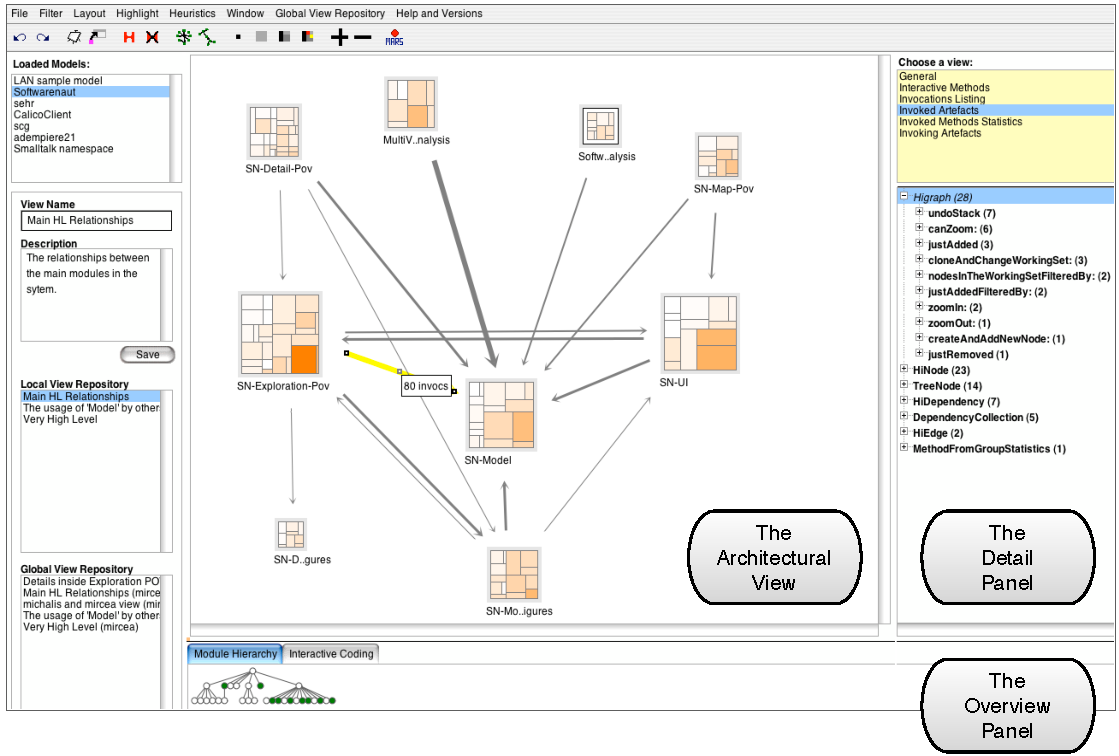
\includegraphics[width=0.8\linewidth]{images/SnautOnSnaut}
\caption{Softwarenaut uses linked views to present multiple perspectives on a software system at once}
\flabel{sos}
\end{center}
\end{figure}

The UI of Softwarenaut is composed of three linked complementary visual perspectives that present information about the system during the exploration. \fref{sos} presents Softwarenaut visualizing an architectural view of itself. The figure illustrates the three complementary views that the tool supports:

\begin{enumerate}
\item The Exploration View. The Exploration View is the main view in Softwarenaut. It is a graph-based representation of modules and their dependencies. The modules are represented as nodes in the graph and their dependencies are rep- resented as directed edges between the modules. Each dependency edge is an aggregation of low-level dependencies between the two associated modules.
\item The Detail View. This view presents details for the entity that is currently selected in the Exploration View. The goal of this view is to provide insight into the details of the element selected in the exploration view.
\item The Overview View. The overview view presents the entire hierarchy of the system and highlights on it the modules that are currently visible in the exploration view. The Overview view presents a horizontal slice through the system \cite{wong-thesis}. The view is interactive: the user can navigate to the details of the elements in the view, or select elements in the detailed view and have the selection propagate to the exploration view. This view is significant because it offers a sense of orientation during the top-down navigation.
\end{enumerate}


Like other architecture recovery tools, Softwarenaut is organized along a classical extract-abstract-view workflow as presented in \fref{flow}.

\begin{figure}[h]
\begin{center}
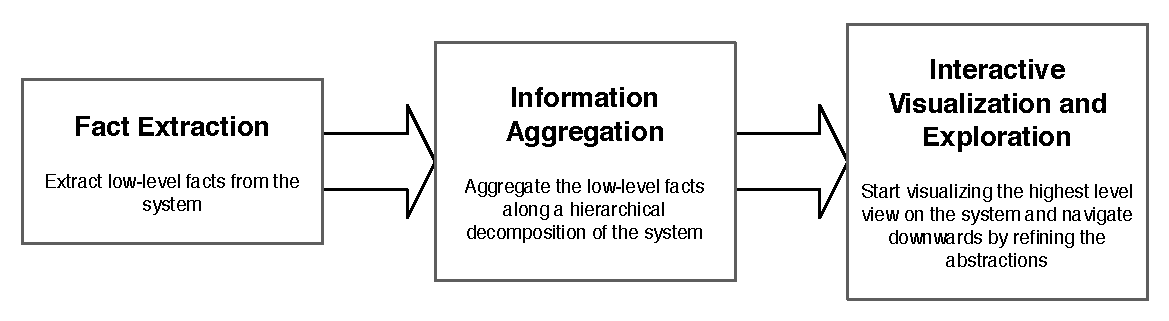
\includegraphics[width=\linewidth]{images/SnautFlow}
\caption{Softwarenaut supports an extract-abstract-view workflow model}
\flabel{flow}
\end{center}
\end{figure}

In the remainder of this article we will dedicate to each of the three steps of the workflow an entire section. 




\newpage
% FACTS
\section {Fact Extraction}
\label{sec:facts}

The first step in architecture recovery is fact extraction. 

There are two types of facts that one can extract from the source code: artifacts, and relationships between them. 

Softwarenaut is built on top of FAMIX, a language independent object-oriented software meta-model...
FAMIX is a meta-model that supports the representation of systems written in object-oriented languages. Softwarenaut takes as input the model of a software system as it can be represented by FAMIX (specifically FAMIX 2.0). 


\subsection {Horizontal Relationships between Software Artefacts}

Depending on what are the extracted artefacts, and what is the language that is analyzed the dependnencies between artefacts can be of various types:

include relationships between files in C/C++
subclassing relationships between classes in all the Object Oriented languages
invocations between methods or functions in any programming language

The FAMIX model can model all these, and some more.


\subsection {Vertical Relationships between software artifacts}

Hierarchical organization is one of the most powerful tools for managing complexity. In software this means that in most of the cases, a software system is organized hierarchically: methods are grouped in classes, classes are grouped in modules, modules in systems. The relationships between artefacts that organize the system in a vertical hierarchy are called vertical relationships between the software artefacts. 

At the architectural level, various languages provide different mechanisms for the hierarchical organization of the system. In C/C++ the organization is given by the directory structure of the project, in Java by the package hierarchy, in Cincom Smalltalk by the bundles hierarchy, etc. In the cases where there is no hierarchy in place one can be automatically generated by performing hierarchical clustering on the artefacts in the system [LunguKuhnLongTimeAgo]. 



\newpage
% ORGANIZATION
\section {Information Aggregation}
\label{sec:org}

Aggregating horizontal relationships between software artefacts along vertical relationships is the fundamental technique that allows for abstraction in Softwarenaut. A data structure that allows for this is the Higraph\cite{harel-visform}. The Higraph is a data structure formed by taking the graph of basic artefacts and horizontal relationships that exist between them and aggregating and propagating those relationships upwards along the hierarchical decomposition of the system. 

Figure \ref{dep-agg} presents the process through which the low-level horizontal relationships between the methods of classes in a Java system are aggregated up along the hierarchical decomposition of the system. There are two explicit horizontal dependencies that are extracted from the system: the method calls between \cod{mc1} and respectively \cod{mc2} and \cod{mc5}. 
The explicit dependencies are propagated as implicit relationships vertically along the vertical relationships \cod{mc1 -- c1 -- B -- A}, \cod{mc5 -- c5 -- d -- c} and \cod{mc2 -- c2 -- d --c}. The highest level implicit relationship is the one between A and C. 


\begin{figure}[h]
\begin{center}
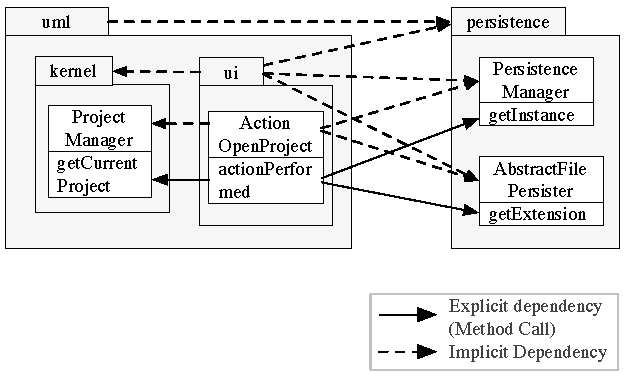
\includegraphics[width=0.8\linewidth]{images/DependencyAggregation}
\caption{The aggregation of explicit dependencies into implicit ones along the vertical relationships between methods, classes, and packages in a Java system}
\label{dep-agg}
\end{center}
\end{figure}

When a hierarchical decomposition is not provided, we can automatically generate one using clustering techniques. We presented elsewhere an experiment with clustering the classes in a system based on the similarity in the natural language terms that are used in their definitions \cite{Lung05a} and there is a rich literature on clustering software systems in general \cite{koschke-thesis}.

\begin{figure}[h]
\begin{center}
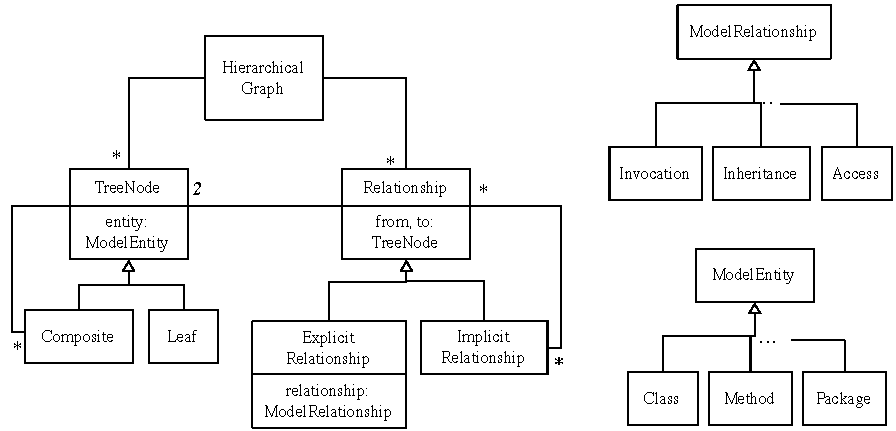
\includegraphics[width=0.7\linewidth]{images/HigraphModel}
\caption{The DPMHigraph model is the core representation of a system in Softwarenaut}
%DPM stands for Detailed Project Model
\flabel{hmodel}
\end{center}
\end{figure}


The diagram from \fref{hmodel} presents two types of abstract entities and two types of abstract relations:
\begin{itemize}
\item Leaf Entities. The leaf entities are the basic object-oriented programming building blocks used for the structuring of software. Depending on the analyzed relation- ship, the leaf entities can be either methods or classes.
\item Composite Entities. The composite entities are containers for other entities. They can have direct mappings to programming language entities, such as classes, packages, namespaces or modules but can also represent abstract composites such as clusters.
\item Explicit Relationships. These are the relations between two entities. They are extracted from the code. The ones that we are interested in are method invocations, class inheritance and field access.
\item Implicit Relationships. The model admits relationships between any abstract entities. However, in software systems explicit relationships usually exist only be- tween the leaf entities. Therefore, the relations between the composite entities are inferred bottom-up from the relations existing between the leafs. The result is that between any two high-level components, we have a relation that represents a collection of all the relations between the leaf components aggregated in them.
\end{itemize}




% INTERACTION
\section {Interactive Exploration}
\label {sec:interact}

In this section we detail the interactive techniques that support the exploration process in Softwarenaut: higraph navigation, rule-based filtering, first-class views, and details-on-demand.  

\subsection{Navigation}
The dominant exploration mechanism of Softwarenaut is refinement. One starts with a very high-level abstracted view of a system and he continuously refines by using exploration operations [RMC91]. At a given moment the set of visible nodes with which the user interacts constitutes the working set (WS). Initially the working set contains very few nodes and they are very high-level. As the useress explores the system she transforms the working set by performing exploration operations on it. 


\begin{figure}[b!]
\begin{center}
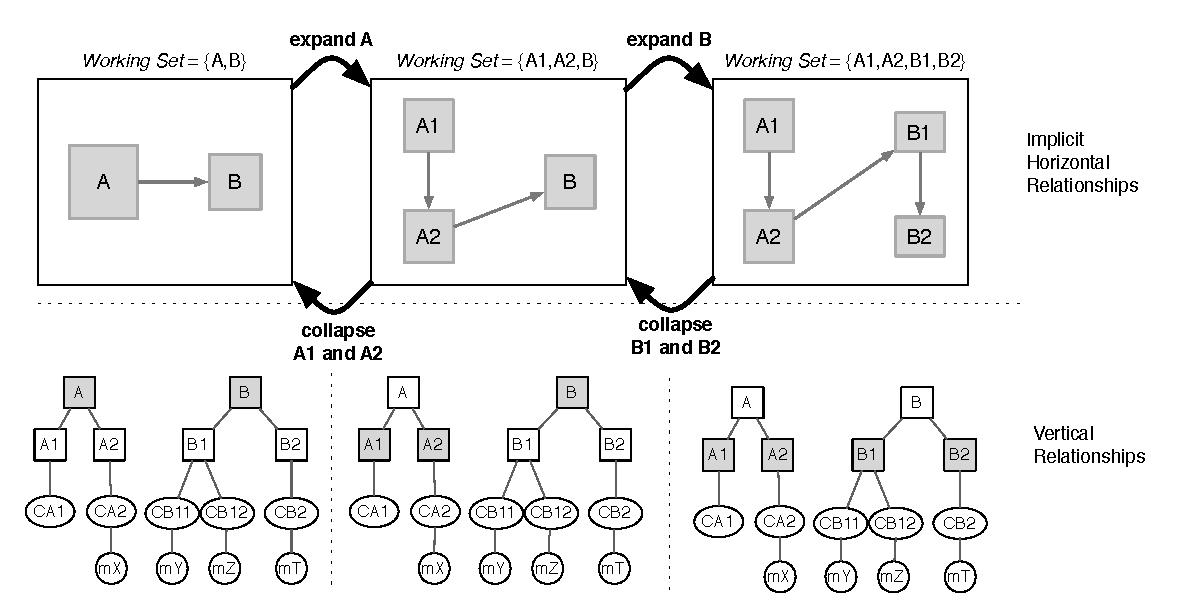
\includegraphics[width=\linewidth]{images/SnautSequence}
\caption{The expand and collapse complementary operations that allow vertical navigation in the Higraph}
\label{}
\end{center}
\end{figure}

The exploration operations that are supported by Softwarenaut are:

\begin{itemize}

\item Expand. By applying the expand operation to a node of the working set, the node is replaced in the working set with nodes representing its children. The operation can be represented in set notation in the following way:

ExpandN(WS)= WS − N + children(N), where children (N) is a function 	which returns the children of the node N in the reference higraph.

\item Collapse. By collapsing a node corresponding to a module, the node, together with all the nodes representing the siblings of the module are removed from the view and replaced with a node representing the parent module. In set notation the operation is represented as follows:

CollapseN (WS) = WS − N − siblings(N) + parent(N)

\item Filter.
By filtering a node, that node (and implicitly its children) will be removed from the working set. In set notation the operation is represented as follows:

FilterN(WS)=WS−N


\item Group.
By grouping several nodes together the user can reduce the clutter in the view. 

GroupNi,I<G(WS) = WS - Ni,I<G + NewGroup


\end{itemize}

As the user refines the view, and climbs down in the hierarchy of the system, more and more elements are brought into the view. In order to cope with this complexity the user can use the Filter and Group operations on individual nodes. Individual nodes that usually benefit from being filtered out are the “omnipresent suppliers” utility nodes that provide functionality to the majority of the elements in the view. Usually they provide little to the understanding of the architecture of the system, but they make the view really cluttered. 


\newpage
\subsection {Details-on-Demand}

The information visualization mantra is “overview first, zoom and filter, and details on demand” 

Having arrived at an architectural view, in Softwarenaut is the beginning of the process of understanding that view. If the view were a story, then the nodes in the view are its nouns and the edges are the verbs in a sentence. Only when one has recovered the meaning of the all the verbs and the nouns he can say that he has really understood the story of the view. The details-on-demand panel of Softwarenaut is one of the ways in which one can understand the individual nodes and edges in the Architectural View.


\subsubsection {Details for Edges}
They present the history of the edges, when multiple veresions of the system are available (an example of a detailed view is the Evolution filmstrip [EF06] that is presented in Figure XXX) and structural informations when a single version of the system is available. 

\begin{figure}[h]
\begin{center}
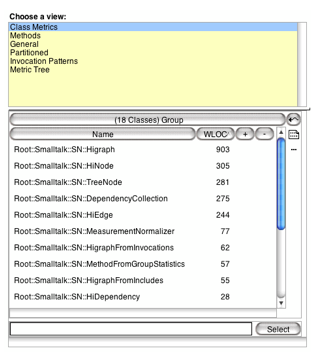
\includegraphics[width=0.5\linewidth]{images/DetailForNode.png}
\caption{}
\label{}
\end{center}
\end{figure}
Figure XXZ presents a detailed view of the “Invoked Artefacts” detail view. The tree has on its first levels the names of the classes that are invoked in the invocations that are abstracted in the dependency. Besides each node is the number of methods that are invoked from that class. The figure also presents one node (Higraph) being expanded and it shows the individual methods that are invoked from that class. The method nodes can be further expanded and the call sites can then be revealed. 


\subsubsection {Details for Nodes}

They present details about the selected node entity. The bottom part of Figure XXY presents the “Class Metrics” detail-view. It lists all the classes that are aggregated in a certain module and it can display metrics for them. The figure shows the list of classes in the SN-Model module that is part of the Softwarenaut itself. The classes are sorted based on their size. One can add new metrics that are visualized, or can navigate to the code of the individual classes from this panel.

\begin{figure}[h]
\begin{center}
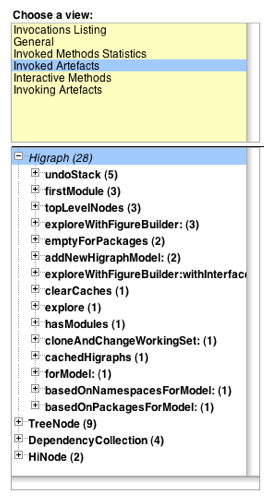
\includegraphics[width=0.4\linewidth]{images/DetailForEdge.png}
\caption{}
\label{}
\end{center}
\end{figure}


\subsection {Rule-Based Filtering}

In the previous section we have introduced the Filter and Group operations which work on individual nodes. A complementary type of filtering is rule-based filtering. There are several types of such filters:

\begin{itemize}
\item Metric-based filters. Filtering entities and relationships based on their properties. One example of this is filtering the weak dependencies or filter- ing the modules that do not depend on others.
\item Type-based filters. Filtering entities or relations of a given type. One example of this is showing only inheritance relationships, or filtering out the classes in a system.
\end{itemize}

\begin{figure}[ht!]
\begin{center}
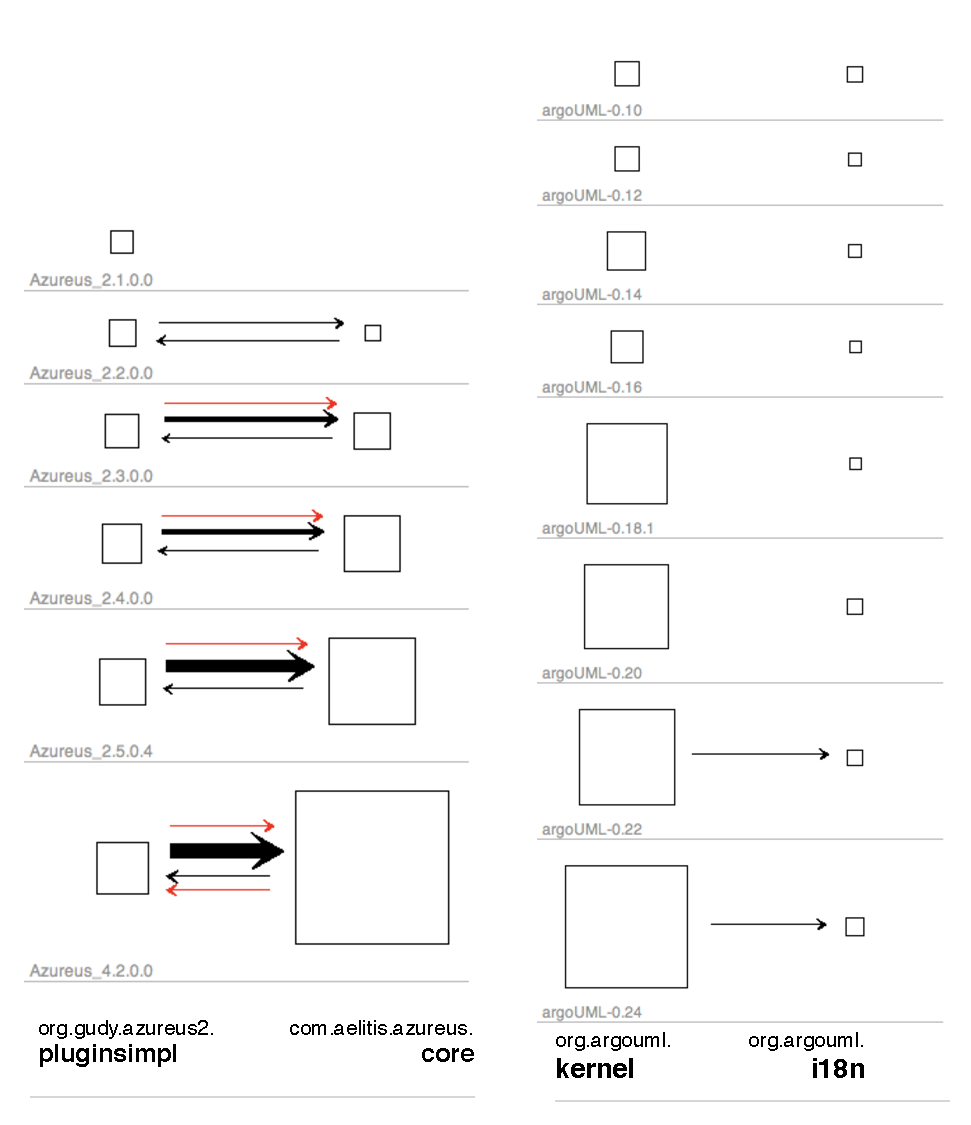
\includegraphics[width=0.7\linewidth]{images/Filmstrip}
\caption{}
\label{}
\end{center}
\end{figure}


When it comes to filtering there are two types of filters: deep filters and shallow filters.

\begin{itemize}

\item Low-level Filters. They act on the higraph itself. They remove from the higraph the low-level elements that match a given condition. For example, removing all the invocation relationships that go to polymorphic classes, will not remove the visual dependency between two modules if they contain other types of low-level dependencies.

\item High-level Filters. They act on the high-level elements and relationships between them in the working set. For example, removing from the view all the dependencies that abstract less than 100 explicit dependencies.

\end{itemize}


Figure A.7 presents the relation filtering panel as implemented in Softwarenaut. Several filters can be combined to obtain more powerful ones. During the exploration, the user generates many views. If a filter is active, each time a new view is generated, only those dependencies that the filter allows to be visible are visible.


\begin{figure}[h]
\begin{center}
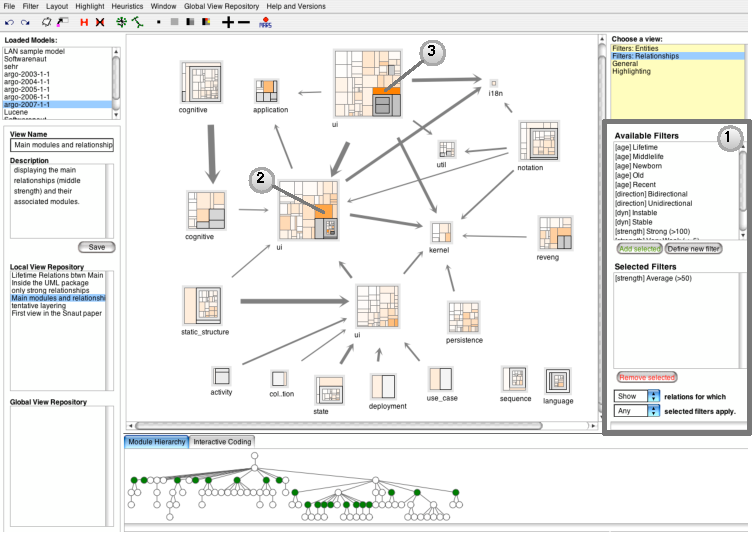
\includegraphics[width=\linewidth]{images/SnautFilteringPanel}
\caption{The UI for applying relationship filters in Softwarenaut}
\label{}
\end{center}
\end{figure}

In the figure one can observe several types of high-level filters that apply on relationships: 

\begin{itemize}
\item Age-based Filters. They are defined based on the historical presence of an inter-module relationship in the system. They can only be applied when models for multiple versions of a system are loaded. Fossil, Old, Lifetime, and Recent are four age-based filters that correspond to relationships which have the properties suggested by their names. In Figure XXY the first relationship is an old one, while the second is a new one. 

\item Dynamics-based Filters. They are defined based on the dynamics of the relationship. Some relationships are stable across the versions while others are continuously changing. Two such filters are Stable and Instable. In Figure XXY the first relatinoship is instable since all during the evolution of the system the types of relationships and their directions change while the second is stable.

\item Directional Filters. They are defined based on the direction of the relationship between two modules. Unidirectional, and bidirectional are such filters and the filter out relationships that correspond to their names. Filtering out the unidirectional relationships from an architectural view is useful for highlighting the modules that have mutual dependencies between themselves. 
\end{itemize}


Rule-based relationships are a powerful way of reducing information in the view. The principle is simple: not all the relationships are equally relevant for the task at hand. When analyzing a system with a specific goal, the analysis will focus first on those relationships that are most relevant for the chosen goal. Two goals that can benefit from such an approach are recovering an architecture and assessing the quality of an architecture:

\begin{itemize}
\item When recovering the architecture of a system, the lifetime and old relationships are more relevant. They represent the architectural backbone of the system and their stability over time insures that it is worth analyzing them first.

\item When assessing the quality of an architecture, the recent relationships are of higher interest. Since they were recently introduced, they are more likely to be contrary to the original intended architecture. They might be the result of archi- tectural decay or of changes to the system performed by new developers that are unaware of the architecture. Continuously monitoring these relationships can be a good quality assurance policy.
\end{itemize}

Figure 7.14 presents two views on the same set of modules as Figure 7.13. The left side presents all the 21 dependencies that existed between the displayed nodes in all the versions of the system. The right part of the figure presents the 36 dependencies that were introduced in the system in the latest version. Both the numbers are very low in comparison with the number of relationships that are present in the last version of the system so both can function as powerful filters.

\begin{figure}[h]
\begin{center}
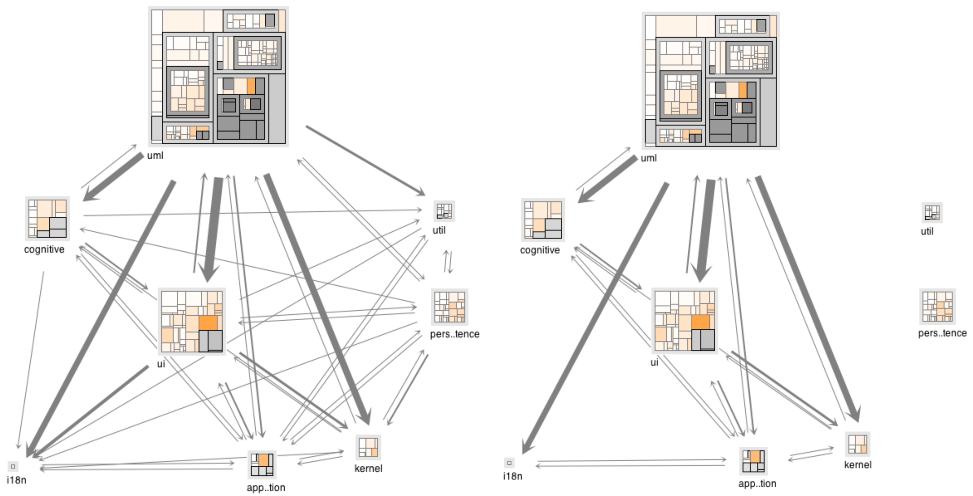
\includegraphics[width=\linewidth]{images/Architecture-LifetimeVsRecent}
\caption{The left part of the figure shows the Lifetime relationships while the right part of the figure presents the Recent relationships in Azureus/Vuze}
\label{}
\end{center}
\end{figure}






\newpage
\subsection {First-Class Views}

Another technique used for avoiding views becoming too complex which can be used in combination with the previously presented techniques is saving views. In fact, there is little hope that a single view can present all the information that is needed for understanding of a complex system. If the designers need different types and multipe diagrams for their understanding, the more will the user that is trying to understand the system. 

There are different approaches that different tools use to cope with this problem. For example, Shrimp and Creole allow zooming in into individual nodes. 

In our case, we allow the saving and restoring of views. Each view can then represent only one perspective on the system. 

Every view is defined by:

\begin{itemize}
\item the current working set
\item the active node filters
\item the active edge filters
\item the current positions of all the visible nodes
\end{itemize}



% COLLABORATION
\section {Collaboration}
\label {sec:collab}

In Softwarenaut, views are entities that can be saved, and shared. One can publish a view in a view repository. Each view is associated with a system or a version of a system. Then, when some other user analyzes that specific system he can download other views that were saved for that system by other users. 

The view repository is based on a Postgres SQL database and saves for each view the following:

\begin{itemize}
\item the creator
\item the system and optionally version of the system for which the view was generated
\end{itemize}

Regarding the filters, at the moment they are predefined. In the future we plan to support user-defined filters and their publication together with the views. 

Figure XXX highlights the way the user can interact with the local views. He has a set of local views that he can save, load, delete locally. Then each of these views he can push to the global view repository. From the global view repository he can pull views, or if he is the creator of such a view he can delete it from the global repository too. For every view the users can discuss and add comments. We have implemented recently the view sharing mechanism and we are eager to test it to see whether it is of such use as we imagine for architecture recovery. 

\begin{figure}[h]
\begin{center}
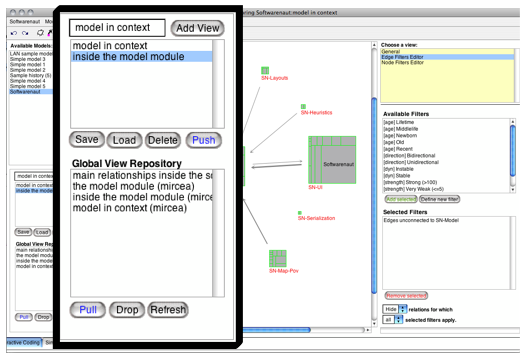
\includegraphics[width=\linewidth]{images/ViewOperations.png}
\caption{}
\label{}
\end{center}
\end{figure}


\subsection {Softwarenaut Synergies}
One of the tools that benefits from the Global View Repository is the Small Project Observatory (abbreviated as SPO). SPO is an ecosystem analysis tool that we have presented elsewhere [SPO]. The goal of SPO is to support the understanding of software ecosystems. We say that SPO works at an abstraction level which is above the architectural level of the individual system, the ecosystem abstraction level. However, in order to understand the  ecosystem the tool needs to support navigatinon between the two abstraction levels. 

One of the tools that benefits from the Global View Repository is the Small Project Observatory (abbreviated as SPO). SPO is an ecosystem analysis tool that we have presented elsewhere [SPO]. The goal of SPO is to support the understanding of software ecosystems. We say that SPO works at an abstraction level which is above the architectural level of the individual system, the ecosystem abstraction level. However, in order to understand the  ecosystem the tool needs to support navigatinon between the two abstraction levels. 


The main use case in which this navigation is needed is when one wants to understand a given system in the context of the ecosystem. In such a case SPO allows navigating down to the architectural level of the individual system, where it presents architectural views which are enriched with information from the ecosystem. The architectural views of the systems are obtained from the Global View Repository where they are published with Softwarenaut. In this way through the two tools can reuse information.

\begin{figure}[th!]
\begin{center}
\includegraphics[width=\linewidth]{images/SpoArchitectural}
\caption{The architectural views saved in Softwarenaut can be imported in SPO}
\label{}
\end{center}
\end{figure}
% This type of view is dynamic, it can not become obsolete...



% DISC
\section {Discussion}
\label {sec:disc}
\subsection {Beyond Reverse Engineering: Monitoring Software Evolution with Softwarenaut}
This is the plan. The future. 

\subsection {Evaluating the Usability and Usefulness of the Tool}
We have tested the tool in two subsequent years with students in our Software Evolution master course. The experiment was a qualitative one where we gave the students an open-source system to analyze after a brief introduction to Softwarenaut. Our goal was to test and get feedback on the usability of the tool as well as its usefullness for reverse engineering large software systems. The students were grouped in pairs and had to analyze ArgoUML and provide a report which presented architectural aspects of the system. We analyzed the results ourselves and found them to be satisfactory of the limited amout of time the students had available. 

Most of the students thought that the tool was easy to use and the results they generated were reliable. The featuers taht they found most useful in their analysis were the details-on-deman views, and the predefined filters. Also most of the students 

The experiment ended with a questionnaire on the features that were missing and the students thought would have made their lives easier. Some of the features that they asked for were: undo/redo facilities, parametrizable filters, arbitrary grouping of classes whose name matches a certain regular expression, 

\subsection {Integration with the Moose Analysis Platform}
Softwarenaut was developed on top of the Moose Analysis Platform. The main feature that the tool uses from Moose is the FAMIX Core meta-model for representing object-oriented systems. The fact that Softwarenaut relies on the FAMIX Core meta-model allows it to be independent of the programming language: as long as there is a fact-extractor from a given language, systems written in that language can be imported and analyzed. 

Softwarenaut also uses several of the views defined in Moose, like for example some of the views that present entity metrics. Also, since behind any visual element of Softwarenaut lays a HiNode and behind it there is a FAMIX entity one can spawn other Moose analyses by selecting any of the elements of a Softwarenaut architectural view. For example, one can select a given module.


\subsection {Beyond Understanding: Reengineering with Softwarenaut}
One of the tools that was built on top of Softwarenaut is MARS: an automated architecture refactoring recommender tool. The tool starts from a given Softwarenaut view and tries to see whether move operations applied on classes can improve the architecture of the system by increasing coupling and decreasing cohesion. The work is still in progress and needs a formal validation. 


% REL
\section {Related Work}
\label {sec:rel}
\subsection {Collaboration.} The work of D’Ambros et. al on the Web-based analysis framework called Churrasco is related in a way to the collaboration part that we support with the architectural view sharing. 

\subsection {Exploration and Navigation.} The first tool that supported this kind of top-down exploration was Shrimp by Storey. However, the tool was intended only for reverse engineering. Our tool, with the facility of first-class views makes a smooth transition towards integrating the views that are once recovered in the forward engineering process of the companies.

Automatically aggregating the low-level relations, and then letting the user navigate from the highest abstraction level downwards is the main interaction approach in Softwarenaut. This is the exact opposite of the approach that M{\"u}ller proposed with Rigi \cite{muller-revengenv}. In their case, the user starts from the lowest-level facts and aggregates them as he climbs up in the abstraction hierarchy. Their approach does not scale when analyzing very large systems because the number of low-level artifacts is too large. Storey took the same top-down navigation approach in her work on SHriMP \cite{storey-shrimp}.

\subsection {First-Class Views.} The work of Storey et al. on Shrimp also allows for saving and restoring views. The views are saved inside a “Filmstrip” and then the filmstrip can be persisted and restored from the disk. Through the intermediation of the filmstrips the users can restore exploration sessions or even share certain views. This type of information allows people that know about each other to share information by emailing the files. The advantage of the Global View Repository is that it allows for discovering information that other users have discovered and about which the analysis is not aware. 
%(http://www.thechiselgroup.org/shrimp_manual_filmstrip)

\subsection {Filtering.} Most of the architecture recovery tools support filtering. There was a paper that surveyed all the techniques. None of the tools however, allows for the users to customize and define filters themselves. That is part of our future work. 


% CONC
\section {Conclusions and Future Work}
\label {sec:conc}
The tool is available online at http://lungu.org/mircea/softwarenaut.











%% The Appendices part is started with the command \appendix;
%% appendix sections are then done as normal sections
%% \appendix

%% \section{}
%% \label{}

%% References
%%
%% Following citation commands can be used in the body text:
%% Usage of \cite is as follows:
%%   \cite{key}          ==>>  [#]
%%   \cite[chap. 2]{key} ==>>  [#, chap. 2]
%%   \citet{key}         ==>>  Author [#]

%% References with bibTeX database:

\bibliographystyle{model1-num-names}
\bibliography{scg,thesis}

%% Authors are advised to submit their bibtex database files. They are
%% requested to list a bibtex style file in the manuscript if they do
%% not want to use model1-num-names.bst.

%% References without bibTeX database:

% \begin{thebibliography}{00}

%% \bibitem must have the following form:
%%   \bibitem{key}...
%%

% \bibitem{}

% \end{thebibliography}


\end{document}

%%
%% End of file `elsarticle-template-1-num.tex'.
